\newpage
\section{Traces des utilisateurs dans les MMOGs}
	\label{trace}
 	Après avoir exposées des solutions qui ne prennent pas en compte la mobilité des joueurs, nous allons étudier cette mobilité pour introduire la solution proposé par le travail Blue Banana. Pour étudier la mobilité dans les MMOGs,différentes techniques de collecte de traces ont été mises en place, nous présenterons celles-ci et expliquerons pourquoi ce travail de collecte est important pour améliorer les performances des solutions pair à pair pour les MMOGs.
	\subsection{Les différentes techniques de récupération de trace}
		\subsubsection{Les objectifs et les techniques de collecte de trace}
		\par Dans la littérature, il y a plusieurs études des traces d'utilisateurs de différents environnements virtuels~\cite{1326262,0295-5075-88-4-48007}. La plupart vont récupérer les traces des avatars sur des jeux vidéos tel que World Of Warcraft~\cite{wow} et Second Life~\cite{sl}. Ces études expliquent qu'il peut y avoir des différences entre des MMOGs. Par exemple dans Second Life l'environnement est beaucoup plus interactif (possibilités plus étendues de modification de l'environnement) que dans World Of Warcraft, ce qui peut affecter des différences de résultats des solutions en fonction du jeu~\cite{DBLP:journals/corr/abs-0807-2328,1613041}. \\
\par Ces travaux permettent de bien comprendre les différents comportements des joueurs, ils permettent ainsi de détecter les différents comportements en fonction des zones plus ou moins peuplées. Grâce à ces travaux, il est possible de faire ressortir des modèles montrant le comportement des avatars dans le monde virtuel. Ces modèles permettent de mettre en place une distribution spatiale des avatars, qui sera plus cohérente que dans les recherches où les distributions étaient uniformes~\cite{Knutsson04peer-to-peersupport}. Différentes mesures vont apparaître comme: le nombre de joueurs, le nombre d'arrivées et de départs, le temps moyen d'une session, la distribution des joueurs, etc. L'étude des traces des joueurs permet aussi de détecter les tricheurs qui utilisent souvent des bots~\cite{0295-5075-88-4-48007}. \\
		%\subsubsection{Les techniques de collecte des traces}
	\par Certaines techniques utilisent un bot qui est introduit dans le jeu et qui va récupérer des informations sur les autres joueurs. Le bot va rapatrier des informations à intervalles réguliers, il sera alors possible d'analyser les déplacements et vérifier les modèles. Une librairie open source \textit{libsecondlife} a été développée pour collecter les traces des joueurs de Second Life, à l'aide d'un bot~\cite{DBLP:journals/corr/abs-0807-2328}. Pour vérifier que les données récupérées sont cohérentes, une technique de positionnement de sept bots dans une région a été mise en place. Quatre bots statiques sont placés à chaque coin de la région, un autre statique va se placer au centre et deux autres vont bouger suivant un schéma défini. Il est alors possible d'enregistrer les positions des avatars se trouvant dans la région et les enregistrements des informations seront réalisés sept fois (par chaque bot). Une comparaison des données des sept bots est alors effectuée pour voir si des déviations existent entre les valeurs et si elles sont importantes.\\  
 		\subsubsection{Limitations de la collecte des traces}
	Des limitations existent pour la collecte des traces. Une des premières est que les mondes virtuels sont très souvent découpés en région ou en île, or les bots que nous introduisons ne peuvent pas traverser les régions et ils ne peuvent pas, par exemple, suivre des avatars. Dans certaine étude~\cite{DBLP:journals/corr/abs-0807-2328}, la possibilité de différencier un avatar qui va dans une autre région et un qui quitte le jeu n'est pas possible. Il n'est pas possible de savoir ce que va faire l'avatar en dehors de la zone. Il y aussi un problème avec la détection des avatars qui se trouvent sur des objets et il n'y pas de prise en compte de la coordonnée \textit{z}. Une autre limitation de la collecte des traces est qu'elle se fait en très grande majorité de façon manuelle, il est donc très long et fastidieux de récupérer un nombre de traces suffisant pour effectuer des bonnes analyses. La collecte de trace peut aussi avoir des problèmes de passage à l'échelle car les systèmes de collecte existants travaillent à une petite échelle. Par exemple dans Second Life, le monde étant découpé en îles indépendantes, l'addition des traces collectées sur chaque île pour en faire une étude globale, n'est pas cohérente.

	\subsection{Observations des traces}
	 Beaucoup d'observations sur les déplacements des avatars dans les mondes virtuels ont pu être réalisé grâce à la collecte de toutes ces traces. La collecte des traces a aussi permis de faire valider ou invalider des modèles qui avaient été mis en place sans étude des traces~\cite{DBLP:journals/corr/abs-0807-2328}. 
		\subsubsection{Hotspots}
	Les études des traces ont permis de faire ressortir l'existence de différentes zones dans le monde. Une autre observation est que les mouvements des avatars sont très différents en fonction de la zone où ils se trouvent. Deux types de zones peuvent se dégager: des zones très peuplées avec des avatars ayant des mouvements très aléatoires et lents (Hotspots), et des zones qui sont entre les zones peuplées, où les avatars se déplacent rapidement et suivent souvent une trajectoire rectiligne (Waypoints). Des phénomènes de déplacement en groupe ont aussi pu être repérés~\cite{15141312}. \\
		\subsubsection{Waypoints}
	Le schéma~\ref{sch_trace} permet de mettre en évidence la présence de ``routes'' entre les différents points de regroupement. Ces routes vont nous permettre de mieux anticiper les déplacements des avatars entre les \textit{Hotspots}.
        \vspace{1mm}
        \begin{figure}[!h]
        \centering
        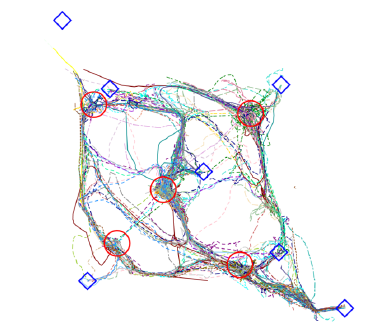
\includegraphics[scale=0.75]{./Ressources/Images/trace.png}\\
        \caption{Battle 980 movement paths}
        \label{sch_trace}
        \end{figure}	
        \vspace{1mm}
\newline
	L'étude des traces a aussi permis de détecter les habitudes des joueurs, comme le fait qu'ils jouent à certaines heures plutôt que d'autres et avec des durées de connexion différentes en fonction de l'heure de la journée.
